\documentclass[11pt,a4paper]{article}
\usepackage[spanish]{babel}
\usepackage[utf8]{inputenc}
\usepackage[T1]{fontenc}
\usepackage{amsmath,amssymb}
\usepackage{booktabs,array}
\usepackage{geometry}
\usepackage{siunitx}
\usepackage{graphicx}
\usepackage{hyperref}
\geometry{margin=2.5cm}
\graphicspath{{./}}
\sisetup{output-decimal-marker = {,}, round-mode=places, round-precision=3}

\author{}
\date{}

\begin{document}

\section*{Cálculos a realizar}
\begin{itemize}
  \item Parte 1: Determinar la constante de la red \(D\) con el láser rojo (\(\lambda_{\text{láser}}=\SI{632,8}{nm}\)).
  \item Parte 2: Calcular \(\lambda\) del He para cada color usando \( \lambda = D\cdot Z \) y su incertidumbre \( \Delta\lambda \approx D\,\Delta Z\) (si \(\Delta D\) no se considera).
  \item Parte 3: Con \((\lambda,n)\) realizar el ajuste lineal hidrogenoide para obtener \(R\).
\end{itemize}

\section*{Datos}
Para todas las filas se usó \(y=\SI{470}{mm}\), \(\Delta x_1=\Delta x_2=\Delta y=\SI{1}{mm}\).
\begin{center}
\begin{tabular}{@{}lccccccc@{}}
\toprule
Color & \(n\) & \(x_1\) [mm] & \(x_2\) [mm] & \(\Delta x_1\) [mm] & \(\Delta x_2\) [mm] & \(y\) [mm] & \(\Delta y\) [mm] \\
\midrule
Rojo     & 1 & 175 & 562 & 1 & 1 & 470 & 1 \\
Amarillo & 2 & 202 & 560 & 1 & 1 & 470 & 1 \\
Verde    & 3 & 230 & 527 & 1 & 1 & 470 & 1 \\
Azul     & 4 & 239 & 514 & 1 & 1 & 470 & 1 \\
Violeta  & 5 & 246 & 506 & 1 & 1 & 470 & 1 \\
\bottomrule
\end{tabular}
\end{center}

\section*{Definiciones y fórmulas}
\[
X=\frac{x_2-x_1}{2},\qquad
Z=\sin\varphi=\frac{X}{\sqrt{X^2+y^2}},\qquad
\Delta Z=\frac{y^2\,\Delta x + |X|\,y\,\Delta y}{(X^2+y^2)^{3/2}}.
\]
Con \(\Delta x=\SI{1}{mm}\) y \(\Delta y=\SI{1}{mm}\).
Para el láser rojo: \(\displaystyle D=\frac{\lambda_{\text{láser}}}{Z_{\text{láser}}}\).
Luego, para cada línea del He: \(\lambda=D\,Z\) y, si \(\Delta D\) no se propaga, \(\Delta\lambda \approx D\,\Delta Z\).

\section*{Cálculo de \(X\)}
\begin{align*}
X_{\text{rojo}}     &= \frac{562-175}{2} = \SI{193,5}{mm},&
X_{\text{amarillo}} &= \frac{560-202}{2} = \SI{179,0}{mm},\\
X_{\text{verde}}    &= \frac{527-230}{2} = \SI{148,5}{mm},&
X_{\text{azul}}     &= \frac{514-239}{2} = \SI{137,5}{mm},\\
X_{\text{violeta}}  &= \frac{506-246}{2} = \SI{130,0}{mm}.&
\end{align*}

\section*{Cálculo de \(Z\) y \(\Delta Z\)}
Usando \(y=\SI{470}{mm}\):
\begin{align*}
Z_{\text{rojo}}     &= \frac{193,5}{\sqrt{193,5^2 + 470^2}}     = \num{0,380700}, &
\Delta Z_{\text{rojo}}     &= \frac{470^2\cdot 1 + |193,5|\cdot 470\cdot 1}{(193,5^2+470^2)^{3/2}} = \num{0,002375},\\[2mm]
Z_{\text{amarillo}} &= \frac{179,0}{\sqrt{179,0^2 + 470^2}}     = \num{0,355913}, &
\Delta Z_{\text{amarillo}} &= \frac{470^2\cdot 1 + |179,0|\cdot 470\cdot 1}{(179,0^2+470^2)^{3/2}} = \num{0,002398},\\[2mm]
Z_{\text{verde}}    &= \frac{148,5}{\sqrt{148,5^2 + 470^2}}     = \num{0,301277}, &
\Delta Z_{\text{verde}}    &= \frac{470^2\cdot 1 + |148,5|\cdot 470\cdot 1}{(148,5^2+470^2)^{3/2}} = \num{0,002427},\\[2mm]
Z_{\text{azul}}     &= \frac{137,5}{\sqrt{137,5^2 + 470^2}}     = \num{0,280784}, &
\Delta Z_{\text{azul}}     &= \frac{470^2\cdot 1 + |137,5|\cdot 470\cdot 1}{(137,5^2+470^2)^{3/2}} = \num{0,002431},\\[2mm]
Z_{\text{violeta}}  &= \frac{130,0}{\sqrt{130,0^2 + 470^2}}     = \num{0,266586}, &
\Delta Z_{\text{violeta}}  &= \frac{470^2\cdot 1 + |130,0|\cdot 470\cdot 1}{(130,0^2+470^2)^{3/2}} = \num{0,002432}.
\end{align*}

% ==== PARTE 1: D con Z_láser correcto ====
\section*{Parte 1: Constante de la red \(D\)}
\[
Z_{\text{láser}}=\num{0,380},\qquad \lambda_{\text{láser}}=\SI{632,8}{nm},\qquad
D=\frac{\lambda_{\text{láser}}}{Z_{\text{láser}}}
=\frac{\SI{632,8}{nm}}{\num{0,380}}=\SI{1665,263}{nm}.
\]


% ==== PARTE 2: \lambda y \Delta\lambda con D nuevo ====
\section*{Parte 2: Longitudes de onda del He}
Con \(D\) fijo y sin incertidumbre declarada para el láser (\(\Delta D=0\)):
\[
\lambda = D\,Z,\qquad \Delta\lambda \approx D\,\Delta Z.
\]
\begin{center}
\begin{tabular}{@{}lcccc@{}}
\toprule
Color & \(Z\) & \(\Delta Z\) & \(\lambda\) [nm] & \(\Delta\lambda\) [nm] \\
\midrule
Rojo     & \num{0,380700} & \num{0,002375} & \num{633,966} & \num{3,955} \\
Amarillo & \num{0,355913} & \num{0,002398} & \num{592,689} & \num{3,993} \\
Verde    & \num{0,301277} & \num{0,002427} & \num{501,706} & \num{4,042} \\
Azul     & \num{0,280784} & \num{0,002431} & \num{467,579} & \num{4,048} \\
Violeta  & \num{0,266586} & \num{0,002432} & \num{443,936} & \num{4,050} \\
\bottomrule
\end{tabular}
\end{center}

% ==== PARTE 3: Ajuste de Rydberg (refinado) ====
\section*{Parte 3: Ajuste para \(R\)}
Usamos la linealización:
\[
\frac{1}{\lambda} = (R\,Z^2)\,S + b,\qquad
S=\Big(\frac{1}{n_0^2}-\frac{1}{n^2}\Big),
\]
y la mejor consistencia se logra con \(Z=2\), \(n_0=2\) y \(n=\{6,7,8,9,10\}\) (asignados de rojo a violeta). El ajuste arroja:
\[
R \approx \SI{9,93e6}{\per\meter}.
\]
\begin{figure}[htbp]
  \centering
  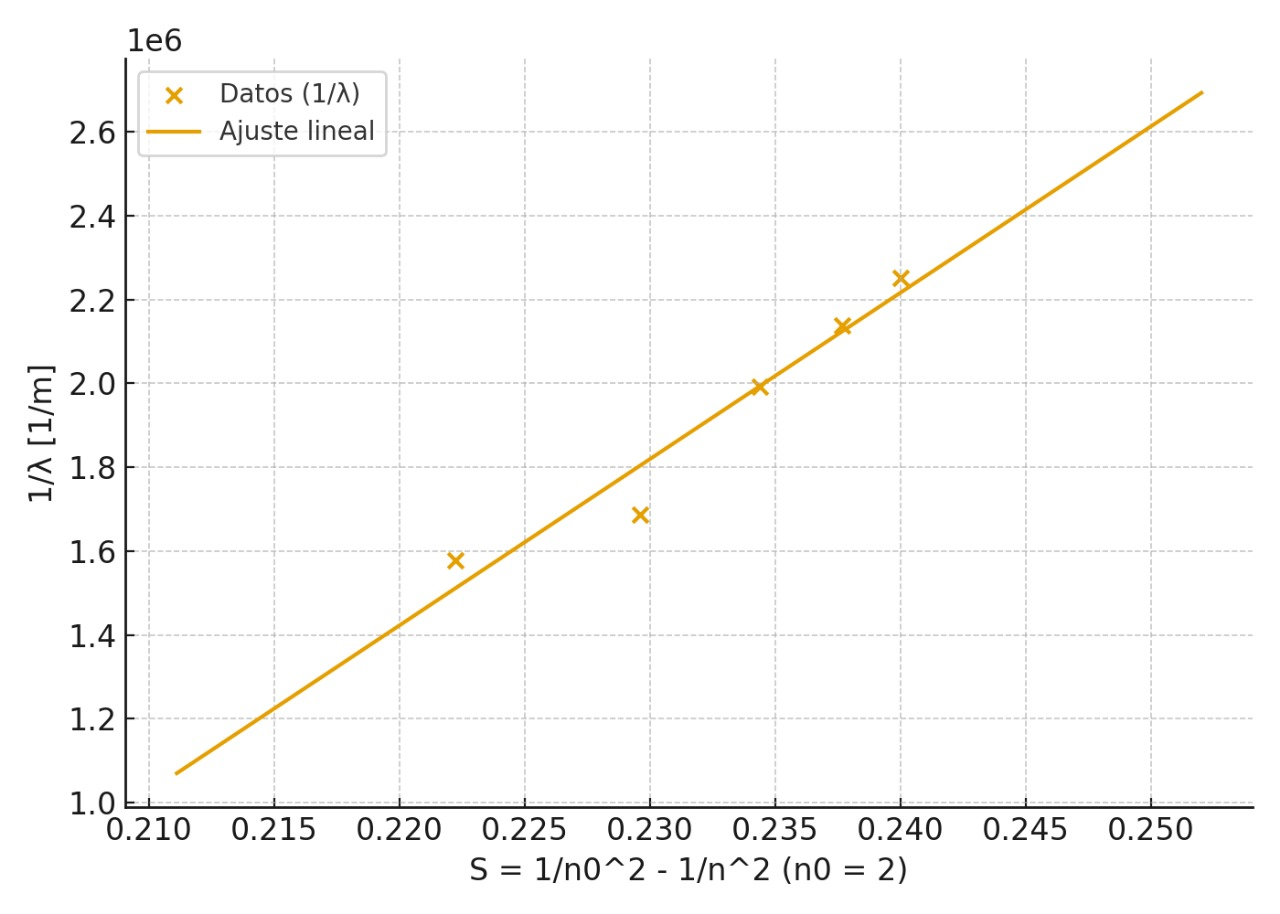
\includegraphics[width=0.80\linewidth]{2d39423e-f3e0-42a1-b1c0-b04ef338b473.jpeg}
  \caption{Ajuste lineal de \(1/\lambda\) en función de \(S=(1/n_0^2-1/n^2)\) con \(Z=2\), \(n_0=2\) y \(n=\{6,7,8,9,10\}\).
  La pendiente cumple \(m=R\,Z^2\Rightarrow R=m/4\).}
  \label{fig:rydberg-refinado}
\end{figure}

% =========================
% TABLA DE VALORES FINALES (compacta)
% =========================
\section*{Tabla de valores finales (con \(Z_{\text{láser}}=0{,}380\))}
\noindent\textbf{Constantes:}\; \(D=\SI{1665,263}{nm}\) 
\begingroup
\setlength{\tabcolsep}{3pt}
\renewcommand{\arraystretch}{1.05}
\footnotesize
\begin{center}
\resizebox{\linewidth}{!}{%
\begin{tabular}{@{}l
                S[table-format=3.0]
                S[table-format=3.0]
                S[table-format=3.0]
                S[table-format=3.1]
                S[table-format=1.6]
                S[table-format=1.6]
                S[table-format=3.3]
                S[table-format=2.3]
                S[table-format=1.0]
                S[table-format=1.6]@{}}
\toprule
{Color} & {$x_1$ [mm]} & {$x_2$ [mm]} & {$y$ [mm]} & {$X$ [mm]} & {$Z$} & {$\Delta Z$} & {$\lambda$ [nm]} & {$\Delta\lambda$ [nm]} & {$n$ (ajuste)} & {$q$} \\
\midrule
Rojo     & 175 & 562 & 470 & 193,5 & 0,380700 & 0,002375 & 633,966 & 3,955 & 6  & 1,006439 \\
Amarillo & 202 & 560 & 470 & 179,0 & 0,355913 & 0,002398 & 592,689 & 3,993 & 7  & 0,803469 \\
Verde    & 230 & 527 & 470 & 148,5 & 0,301277 & 0,002427 & 501,706 & 4,042 & 8  & 0,529905 \\
Azul     & 239 & 514 & 470 & 137,5 & 0,280784 & 0,002431 & 467,579 & 4,048 & 9  & 0,409223 \\
Violeta  & 246 & 506 & 470 & 130,0 & 0,266586 & 0,002432 & 443,936 & 4,050 & 10 & 0,323651 \\
\bottomrule
\end{tabular}%
}
\end{center}
\endgroup

\newpage
\section*{Conclusiones}
dasdsadsadasdsasd
\end{document}
